\documentclass[conference]{IEEEtran}

\usepackage{amsmath,amssymb}
\usepackage{array}
\usepackage{booktabs}
\usepackage{cite}
\usepackage[T1]{fontenc}
\usepackage{graphicx}
\usepackage{microtype}
\usepackage{algorithm}
\usepackage{algpseudocode}
\usepackage{pgfplots}
\usepackage{tikz}
\usepackage{url}
\usepackage{balance}

\pgfplotsset{compat=1.18}
\usetikzlibrary{arrows.meta,positioning}

\title{Q-Learning-Guided Warm-Start LSTM Optimization for ECG Forecasting}

\author{%
\IEEEauthorblockN{Anonymous Author(s)}
\IEEEauthorblockA{Affiliation withheld for blind review\\
Email: author@institution.edu}}

\begin{document}
\maketitle

\begin{abstract}
Selecting the capacity and regularization of a long short-term memory (LSTM) network is a sequential, expensive design problem. This paper formulates compact LSTM configuration search as a Markov decision process and uses tabular Q-learning, driven by the Bellman update, to select the hidden width, recurrent depth, and dropout rate for one-step electrocardiogram (ECG) forecasting. The agent explores 18 configurations through seven local actions. Each selected model is trained for three epochs, and the negative validation mean squared error (MSE) is returned as reward. A warm-start mechanism reuses weights whenever consecutive configurations are structurally compatible; otherwise, training restarts. A recorded CPU experiment on 5,000 ECG5000 traces constructs 600,000 length-20 forecasting windows and evaluates 12 agent episodes. Relative to the notebook's cold-start, manual-SGD search, the Adam-based warm-start search lowers the best MSE from 0.943495 to 0.088472---a 10.66$\times$ reduction---while improving $R^2$ from 0.0759 to 0.9133. At the MSE-selected checkpoint, mean absolute error (MAE) falls from 0.727927 to 0.195127 (3.73$\times$); the lowest observed MAE is 0.193173 (3.77$\times$). These results support efficient sequential refinement, while also showing that the tenfold claim applies to MSE rather than MAE. Limitations concerning window-level splitting, stochastic repetition, and confounded ablation are stated explicitly.
\end{abstract}

\begin{IEEEkeywords}
electrocardiogram, LSTM, Q-learning, Bellman equation, hyperparameter optimization, time-series forecasting, weight reuse
\end{IEEEkeywords}

\section{Introduction}
Electrocardiograms (ECGs) are ordered physiological signals whose local morphology and longer temporal context both matter. Public resources such as PhysioNet \cite{goldberger2000physiobank} and the UCR Time Series Archive \cite{dau2019ucr} have enabled repeatable evaluation of learning algorithms on such signals. Although the ECG5000 benchmark is normally used for classification, a trace can also be converted into a self-supervised forecasting problem: a model receives the preceding samples and predicts the next amplitude. This formulation tests whether a representation captures short-range signal dynamics without using the class label as a target.

Long short-term memory (LSTM) networks \cite{hochreiter1997lstm} remain a natural recurrent baseline because their gated state mitigates vanishing gradients. However, forecast accuracy depends on hidden width, depth, regularization, optimizer, and training budget. Empirical studies of LSTM variants confirm that configuration decisions can materially change performance \cite{greff2017search}. Exhaustive evaluation is undesirable when every candidate requires training a recurrent model.

Hyperparameter optimization (HPO) has therefore moved beyond manual grids. Random search is a strong baseline \cite{bergstra2012random}; Bayesian optimization uses a surrogate of validation performance \cite{snoek2012practical}; and successive-halving methods allocate resources to promising candidates \cite{jamieson2016nonstochastic,li2018hyperband}. BOHB combines model-based selection with bandit allocation \cite{falkner2018bohb}. Reinforcement learning (RL) provides another view: architecture selection becomes a sequence of actions whose reward is validation quality. This idea has been demonstrated at much larger scale by neural architecture search (NAS) \cite{zoph2017nas}.

This work studies a deliberately small, inspectable alternative based directly on the accompanying notebook. Its contributions are threefold:
\begin{itemize}
    \item an 18-state Markov formulation for LSTM width, depth, and dropout, navigated by a seven-action tabular Q-learning agent;
    \item a compatible-weight warm start that continues learning after no-op or shape-compatible transitions, combined with Adam optimization; and
    \item an evidence-aligned analysis of the recorded run: best MSE improves by 10.66$\times$, while MAE improves by 3.73$\times$ at the MSE-selected checkpoint, not 10$\times$.
\end{itemize}

The experiment is a proof of concept rather than a clinical study. In particular, it does not establish that RL alone causes the reported gain; both compared runs already use the Q-learning controller and differ in optimizer and reuse policy.

\section{Related Work}
\subsection{Deep Models for Time Series}
LSTM introduced an explicit memory cell and gates for preserving useful gradients over long sequences \cite{hochreiter1997lstm}. Greff \emph{et al.} later compared major LSTM design variants and emphasized the importance of sound baselines and tuned components \cite{greff2017search}. In time-series classification, LSTM--FCN combines recurrent and convolutional pathways \cite{karim2018lstmfcn}; broad empirical reviews show both the promise and sensitivity of deep architectures across UCR datasets \cite{fawaz2019review}. Forecasting surveys similarly identify recurrent networks as competitive but stress careful preprocessing, validation, and automatic configuration \cite{hewamalage2021rnn,lim2021survey}.

The present work is narrower than these general architectures: it predicts the next standardized ECG amplitude using a single LSTM followed by a linear head. Dropout is part of the search space because it can reduce co-adaptation \cite{srivastava2014dropout}; following the underlying recurrent implementation, it is active only between stacked LSTM layers.

\subsection{Sequential Configuration Search}
Bellman's Markov decision formulation \cite{bellman1957markovian} provides the basis for recursively evaluating sequential choices. Q-learning learns action values without an explicit transition model and converges under standard finite-state visitation conditions \cite{watkins1992q}. NAS uses RL controllers to generate architectures \cite{zoph2017nas}, while ENAS reduces their cost through parameter sharing \cite{pham2018enas}. Network transformation methods likewise reuse weights when modifying architectures \cite{cai2018efficient}. Inspired by these methods, the notebook keeps the controller and design space small enough for a CPU run and reuses a checkpoint only when tensor shapes are compatible. Adam \cite{kingma2015adam} is used in the warm-start variant to adapt step sizes during the short evaluation budget.

The proposed search is best positioned between black-box HPO and full NAS. Random and Bayesian search normally treat a candidate configuration as an independent point. Multi-fidelity approaches make evaluation budget adaptive, while NAS controllers can generate substantially different graphs. Here, each action changes at most one coordinate of a fixed LSTM family. This locality makes transitions interpretable and a tabular value function feasible, but it also means that the agent cannot discover new cell types, skip connections, or feature extractors. The purpose is not to replace general HPO; it is to test whether a Bellman-guided local controller and safe sequential reuse can improve a constrained forecasting workflow.

\section{Methodology}
\subsection{Problem Statement}
Let $\mathcal{D}_{\mathrm{tr}}$ and $\mathcal{D}_{\mathrm{val}}$ be sets of input windows and next-sample targets. An LSTM configuration $\lambda=(H,L,D)$, training procedure $\mathcal{A}$, and parameter vector $\theta$ define a validation loss
\begin{equation}
  \mathcal{L}_{\mathrm{val}}(\lambda,\theta)
  =\frac{1}{|\mathcal{D}_{\mathrm{val}}|}
  \sum_{(\mathbf{X},y)\in\mathcal{D}_{\mathrm{val}}}
  \left(y-f_{\lambda,\theta}(\mathbf{X})\right)^2.
  \label{eq:objective}
\end{equation}
A conventional HPO objective seeks $\lambda^*=\arg\min_{\lambda\in\Lambda}\mathcal{L}_{\mathrm{val}}(\lambda,\mathcal{A}(\lambda))$. In the notebook, however, the parameters of the next candidate may inherit the immediately preceding checkpoint. Candidate quality is consequently a function of both $\lambda$ and the search history. The RL formulation optimizes a finite-horizon return
\begin{equation}
   G_k=\sum_{j=0}^{K-k-1}\gamma^j r_{k+j+1},
   \qquad r_{k+1}=-\mathcal{L}_{\mathrm{val},k+1},
   \label{eq:return}
\end{equation}
for $K=12$ episodes. The practical output is the checkpoint with minimum recorded MSE, rather than the terminal state. This distinction matters because an exploratory action near the end can lower the return while an earlier candidate remains the best deployable model.

\subsection{Forecasting Task and LSTM}
Let a standardized ECG trace be $\mathbf{x}=(x_1,\ldots,x_{140})$. For a window length $w=20$, every valid position creates
\begin{equation}
    \mathbf{X}_{t}=[x_{t-w},\ldots,x_{t-1}],\qquad y_t=x_t.
    \label{eq:window}
\end{equation}
The LSTM processes $\mathbf{X}_{t}$ in order. For compactness, its update is
\begin{align}
 \mathbf{i}_t &= \sigma(W_i x_t+U_i\mathbf{h}_{t-1}+\mathbf{b}_i), \nonumber\\
 \mathbf{f}_t &= \sigma(W_f x_t+U_f\mathbf{h}_{t-1}+\mathbf{b}_f), \nonumber\\
 \mathbf{o}_t &= \sigma(W_o x_t+U_o\mathbf{h}_{t-1}+\mathbf{b}_o), \nonumber\\
 \tilde{\mathbf{c}}_t &= \tanh(W_c x_t+U_c\mathbf{h}_{t-1}+\mathbf{b}_c), \nonumber\\
 \mathbf{c}_t &= \mathbf{f}_t\odot\mathbf{c}_{t-1}+\mathbf{i}_t\odot\tilde{\mathbf{c}}_t, \quad
 \mathbf{h}_t=\mathbf{o}_t\odot\tanh(\mathbf{c}_t),
 \label{eq:lstm}
\end{align}
and a linear head produces $\hat y_t=\mathbf{w}^{\top}\mathbf{h}_t+b$. Candidate quality is measured by
\begin{equation}
 \operatorname{MSE}=\frac{1}{N}\sum_{n=1}^{N}(y_n-\hat y_n)^2,
 \quad
 \operatorname{MAE}=\frac{1}{N}\sum_{n=1}^{N}|y_n-\hat y_n|.
 \label{eq:metrics}
\end{equation}

\subsection{LSTM Configuration as an MDP}
Each state $s=(H,L,D)$ encodes hidden width, recurrent layers, and dropout:
\begin{equation}
H\in\{32,64,128\},\quad L\in\{1,2\},\quad D\in\{0,0.2,0.4\}.
\end{equation}
The resulting space contains 18 states. Seven actions increment or decrement one coordinate, or keep the current state. Boundary actions are clipped, so they may become self-transitions. The deterministic transition operator is denoted $T(s,a)$. Figure~\ref{fig:architecture} connects this controller to the complete forecasting path.

\begin{figure}[t]
\centering
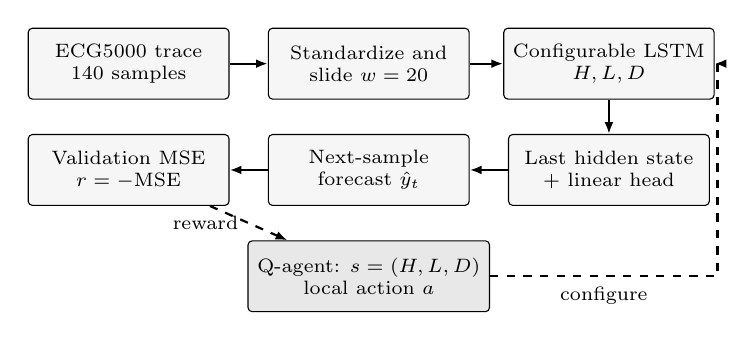
\begin{tikzpicture}[
    block/.style={draw,rounded corners=1.5pt,align=center,font=\scriptsize,
                  minimum width=25.5mm,minimum height=9mm,fill=gray!7},
    control/.style={block,fill=gray!18},
    flow/.style={-{Latex[length=1.5mm]},thick},
    feedback/.style={-{Latex[length=1.5mm]},thick,dashed}
]
\node[block] (signal) at (0,0) {ECG5000 trace\\$140$ samples};
\node[block] (window) at (3.05,0) {Standardize and\\slide $w=20$};
\node[block] (lstm) at (6.10,0) {Configurable LSTM\\$H,L,D$};
\node[block] (reward) at (0,-1.35) {Validation MSE\\$r=-\mathrm{MSE}$};
\node[block] (pred) at (3.05,-1.35) {Next-sample\\forecast $\hat y_t$};
\node[block] (head) at (6.10,-1.35) {Last hidden state\\+ linear head};
\node[control] (agent) at (3.05,-2.70) {Q-agent: $s=(H,L,D)$\\local action $a$};
\draw[flow] (signal)--(window);
\draw[flow] (window)--(lstm);
\draw[flow] (lstm)--(head);
\draw[flow] (head)--(pred);
\draw[flow] (pred)--(reward);
\draw[feedback] (reward)--node[left,font=\scriptsize]{reward} (agent);
\coordinate (cfgturn) at (7.48,-2.70);
\draw[feedback] (agent.east)--node[below,font=\scriptsize]{configure} (cfgturn)|-(lstm.east);
\end{tikzpicture}
\caption{Block-wise architecture of the Q-guided ECG forecaster. Solid arrows form the prediction path; dashed arrows close the search loop.}
\label{fig:architecture}
\end{figure}

After training the LSTM selected by $s'=T(s,a)$, the environment returns $r=-\operatorname{MSE}_{\mathrm{val}}$. The table is updated using the one-step Bellman target:
\begin{equation}
 Q(s,a)\leftarrow Q(s,a)+\alpha\left[r+\gamma\max_{a'}Q(s',a')-Q(s,a)\right],
 \label{eq:qlearning}
\end{equation}
where $\alpha=0.4$ and $\gamma=0.8$. An $\epsilon$-greedy policy with $\epsilon=0.5$ balances exploration and exploitation. All $Q$ values start at zero, the initial state is $(64,1,0)$, and the run lasts 12 episodes.

\begin{figure}[t]
\centering
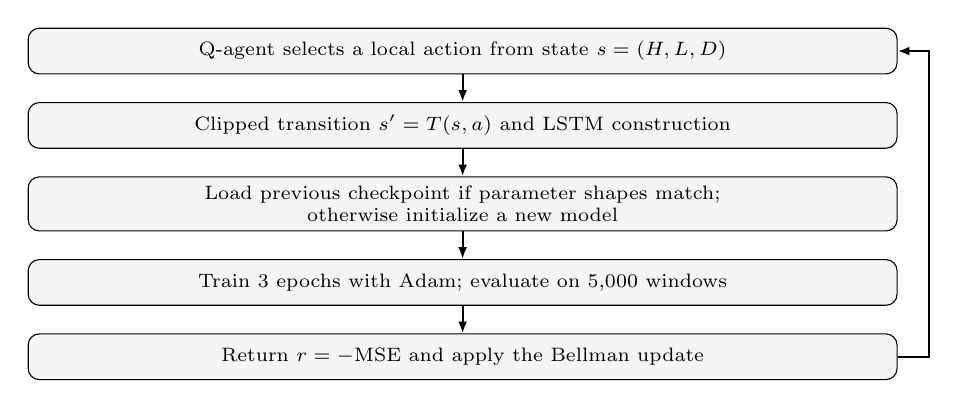
\begin{tikzpicture}[
    node distance=3.5mm,
    box/.style={draw,rounded corners,align=center,font=\scriptsize,minimum width=0.91\columnwidth,minimum height=5.8mm,fill=gray!8},
    arr/.style={-{Latex[length=1.5mm]},thick}
]
\node[box] (agent) {Q-agent selects a local action from state $s=(H,L,D)$};
\node[box,below=of agent] (transition) {Clipped transition $s'=T(s,a)$ and LSTM construction};
\node[box,below=of transition] (reuse) {Load previous checkpoint if parameter shapes match;\\otherwise initialize a new model};
\node[box,below=of reuse] (train) {Train 3 epochs with Adam; evaluate on 5,000 windows};
\node[box,below=of train] (reward) {Return $r=-\mathrm{MSE}$ and apply the Bellman update};
\draw[arr] (agent)--(transition);
\draw[arr] (transition)--(reuse);
\draw[arr] (reuse)--(train);
\draw[arr] (train)--(reward);
\draw[arr] (reward.east) -- ++(4mm,0) |- (agent.east);
\end{tikzpicture}
\caption{One episode of the warm-start Q-learning search.}
\label{fig:pipeline}
\end{figure}

\subsection{Compatible-Weight Reuse}
Figure~\ref{fig:pipeline} summarizes one episode. A candidate model is created first. If its state-dictionary tensor shapes match the preceding checkpoint, all learned parameters are loaded before three further epochs; if loading raises a shape mismatch, the candidate starts from a fresh initialization. Thus, repeated visits to $(128,1,0)$ in episodes 3--6 continue training rather than discarding progress. A change in the nominal dropout value with one recurrent layer is also shape-compatible, although recurrent dropout is inactive when $L=1$. Weight sharing has reduced NAS cost elsewhere \cite{pham2018enas}; here the mechanism is a simpler sequential warm start, not simultaneous supernet sharing.

\begin{algorithm}[t]
\caption{Warm-Start Q-Learning for LSTM Configuration}
\label{alg:warmstart}
\footnotesize
\begin{algorithmic}[1]
\Require $\mathcal{D}_{\mathrm{tr}}$, $\mathcal{D}_{\mathrm{val}}$, state set $\mathcal{S}$, actions $\mathcal{U}$
\Ensure Best checkpoint $b^*$ and episode log $\mathcal{B}$
\State Set $s_0=(64,1,0)$, $Q(s,a)=0$, $\theta^-\gets\varnothing$, $\mathcal{B}\gets\varnothing$
\For{$k=1,\ldots,12$}
    \State Select $a_k$ by an $\epsilon$-greedy policy, $\epsilon=0.5$
    \State Set $s_{k+1}\gets T(s_k,a_k)$ and construct its LSTM
    \State Load $\theta^-$ if parameter shapes match; otherwise reinitialize
    \State Train three epochs with Adam on $\mathcal{D}_{\mathrm{tr}}$
    \State Evaluate MSE, RMSE, MAE, and $R^2$ on $\mathcal{D}_{\mathrm{val}}$
    \State Set $r_k\gets-\mathrm{MSE}_k$ and update $Q$ using \eqref{eq:qlearning}
    \State Save the checkpoint; append $(s_{k+1},a_k,r_k)$ and metrics to $\mathcal{B}$
\EndFor
\State \Return $b^*\gets\arg\min_{b\in\mathcal{B}}\mathrm{MSE}(b)$
\end{algorithmic}
\end{algorithm}

\section{Experimental Protocol}
The notebook downloads the UCR ECG5000 training and test files, concatenates their 5,000 traces, and separates the original class labels from 140-sample signals. A column-wise standard scaler is fitted to the full signal matrix. Equation~\eqref{eq:window} then generates 120 windows per trace, or 600,000 examples. A seeded random 80/20 window-level split forms candidate training and test pools; for CPU feasibility, the first 20,000 training and 5,000 validation examples are retained. Table~\ref{tab:setup} lists the remaining settings.

\begin{figure}[t]
\centering
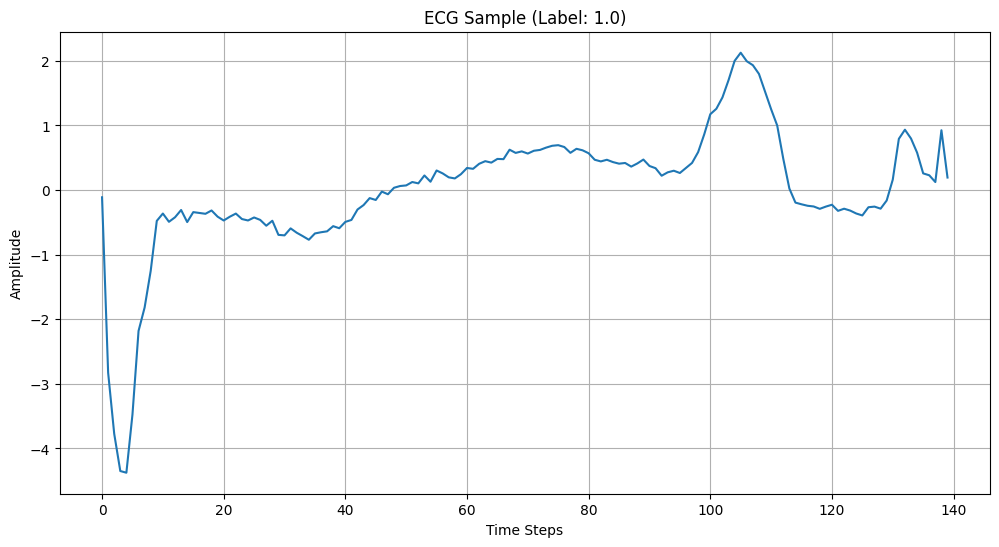
\includegraphics[width=\columnwidth]{figures/ecg_sample.png}
\caption{An ECG5000 trace visualized in the source notebook. The class label is not used by the forecasting target.}
\label{fig:ecg}
\end{figure}

\begin{table}[t]
\caption{Recorded Notebook Configuration}
\label{tab:setup}
\centering
\footnotesize
\begin{tabular}{@{}ll@{}}
\toprule
Setting & Value \\
\midrule
Dataset / traces / length & ECG5000 / 5,000 / 140 \\
Forecast window / target & 20 / next sample \\
Generated / used windows & 600,000 / 20,000 train, 5,000 val. \\
Batch size / device & 512 / CPU \\
Episodes / epochs per episode & 12 / 3 \\
Agent $(\alpha,\gamma,\epsilon)$ & $(0.4,0.8,0.5)$ \\
Warm-start optimizer / rate & Adam / $10^{-3}$ \\
Baseline optimizer / rate & manual SGD / $10^{-3}$ \\
Selection objective & minimum validation MSE \\
\bottomrule
\end{tabular}
\end{table}

The comparison run uses the same agent state/action definitions and reward, but initializes each evaluated LSTM from scratch and applies a manual SGD step for three epochs. The warm-start run uses Adam and the reuse rule above. MSE, root MSE (RMSE), MAE, and $R^2$ are calculated over the validation windows. The notebook does not record wall-clock time, random seeds for model initialization/action selection, repeated trials, confidence intervals, or a held-out final test evaluation; none are inferred here.

In addition to \eqref{eq:metrics}, the recorded metrics are
\begin{equation}
 \operatorname{RMSE}=\sqrt{\operatorname{MSE}},\qquad
 R^2=1-\frac{\sum_n(y_n-\hat y_n)^2}
 {\sum_n(y_n-\bar y)^2}.
 \label{eq:rmser2}
\end{equation}
MSE is the controller's optimization target because it provides a training-aligned measure and penalizes large deviations quadratically. MAE is reported alongside it because its original units and linear penalty offer a complementary view. RMSE must improve by the square root of the MSE ratio; therefore a 10.66$\times$ MSE reduction mathematically corresponds to a $\sqrt{10.66}=3.27\times$ RMSE reduction, not another tenfold change.

\subsection{Model Size and Evaluation Budget}
For input size one and a scalar linear head, a one-layer LSTM has
$4H^2+13H+1$ trainable parameters. A two-layer model has
$12H^2+21H+1$, including both recurrent layers and the head. Table~\ref{tab:params} shows that the design space spans 4,513 to 199,297 parameters. Thus, the state is not merely a label: its width and depth substantially change memory and arithmetic cost. Dropout changes neither parameter count nor tensor shapes.

\begin{table}[t]
\caption{Trainable Parameters by Width and Depth}
\label{tab:params}
\centering
\footnotesize
\begin{tabular}{@{}rrrr@{}}
\toprule
$H$ & $L=1$ & $L=2$ & Two-/one-layer ratio \\
\midrule
32  & 4,513  & 12,961  & 2.87$\times$ \\
64  & 17,217 & 50,497  & 2.93$\times$ \\
128 & 67,201 & 199,297 & 2.97$\times$ \\
\bottomrule
\end{tabular}
\end{table}

With 20,000 training windows and batch size 512, each epoch contains 40 mini-batches (the final one is partial), so an episode performs 120 gradient updates and the 12-episode run performs 1,440 updates across all instantiated models. The recurrent cost of a length-$w$ window is approximately $O(wLH^2)$ when the hidden-to-hidden term dominates. Consequently, a fair large-scale extension should record elapsed time, energy, parameter count, and update budget in addition to forecast error. The current controller optimizes error only and has no incentive to prefer a smaller model when losses are equal.

\section{Results and Discussion}
\subsection{Search Trajectory}
The warm-start agent first selects $(32,1,0)$ and obtains MSE 0.203070. It then moves through 64 and 128 hidden units. When the 128-unit architecture persists, compatible reuse allows cumulative refinement: MSE decreases from 0.134992 at episode 3 to 0.088472 at episode 6, while $R^2$ rises from 0.8678 to 0.9133. Later architecture changes restart training, explaining the temporary degradation in episodes 7 and 8. Selected checkpoints are reported in Table~\ref{tab:trajectory}, and the complete metric curves appear in Fig.~\ref{fig:curves}.

The best-MSE model contains 67,201 parameters, only 33.7\% of the largest candidate's 199,297. The recorded path therefore does not simply reward maximal capacity. Episode 8 evaluates a two-layer, 64-unit model with 50,497 parameters and produces MSE 0.128084, worse than the continuing one-layer, 128-unit model. Because the candidates receive different initialization histories, this observation is descriptive rather than a controlled width-versus-depth ablation.

\begin{table}[t]
\caption{Selected Warm-Start Search Episodes}
\label{tab:trajectory}
\centering
\scriptsize
\setlength{\tabcolsep}{2.1pt}
\begin{tabular}{@{}rcccccc@{}}
\toprule
Ep. & $(H,L,D)$ & MSE & RMSE & MAE & $R^2$ & Reuse \\
\midrule
1  & $(32,1,0)$   & .2031 & .4506 & .2720 & .8011 & No \\
3  & $(128,1,0)$  & .1350 & .3674 & .2471 & .8678 & No \\
4  & $(128,1,0)$  & .0996 & .3156 & .2021 & .9024 & Yes \\
6  & $(128,1,0)$  & \textbf{.0885} & \textbf{.2974} & .1951 & \textbf{.9133} & Yes \\
8  & $(64,2,0)$   & .1281 & .3579 & .2267 & .8746 & No \\
12 & $(64,1,.2)$  & .0910 & .3017 & \textbf{.1932} & .9109 & Yes \\
\bottomrule
\end{tabular}
\end{table}

\begin{figure}[t]
\centering
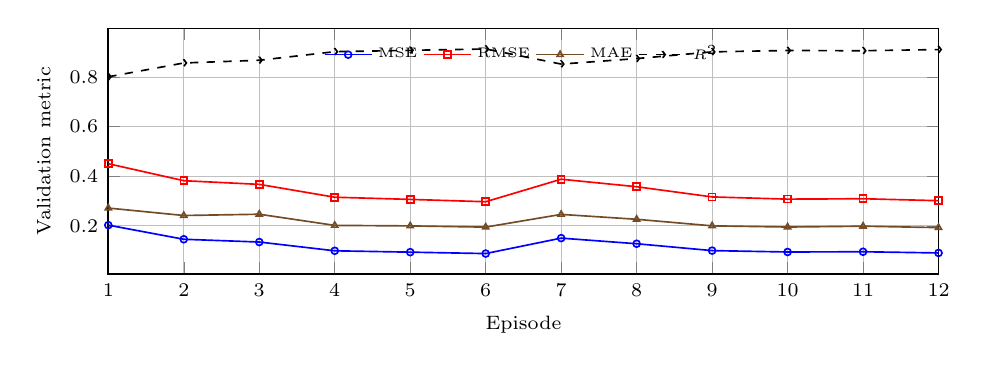
\begin{tikzpicture}
\begin{axis}[
    width=\columnwidth,
    height=4.7cm,
    xmin=1,xmax=12,
    xtick={1,2,...,12},
    xlabel={Episode},
    ylabel={Validation metric},
    grid=major,
    tick label style={font=\scriptsize},
    label style={font=\scriptsize},
    legend style={font=\tiny,at={(0.5,0.98)},anchor=north,legend columns=4,draw=none,fill=none},
    line width=0.6pt,
    mark size=1.25pt
]
\addplot+[mark=o] coordinates {(1,.203070)(2,.146125)(3,.134992)(4,.099625)(5,.094181)(6,.088472)(7,.150709)(8,.128084)(9,.100396)(10,.094838)(11,.095804)(12,.091003)};
\addlegendentry{MSE}
\addplot+[mark=square] coordinates {(1,.450633)(2,.382263)(3,.367413)(4,.315634)(5,.306889)(6,.297443)(7,.388212)(8,.357888)(9,.316853)(10,.307958)(11,.309522)(12,.301667)};
\addlegendentry{RMSE}
\addplot+[mark=triangle] coordinates {(1,.271956)(2,.241944)(3,.247055)(4,.202077)(5,.200000)(6,.195127)(7,.246435)(8,.226655)(9,.200226)(10,.195504)(11,.198827)(12,.193173)};
\addlegendentry{MAE}
\addplot+[mark=diamond,dashed] coordinates {(1,.801106)(2,.856880)(3,.867784)(4,.902424)(5,.907756)(6,.913347)(7,.852391)(8,.874550)(9,.901669)(10,.907112)(11,.906167)(12,.910868)};
\addlegendentry{$R^2$}
\end{axis}
\end{tikzpicture}
\caption{Recorded validation metrics across the 12 warm-start episodes.}
\label{fig:curves}
\end{figure}

\subsection{Magnitude and Meaning of the Improvement}
Table~\ref{tab:comparison} compares the MSE-selected checkpoints. The cold-start/manual-SGD search reaches its best MSE at $(128,1,0.2)$; because this model has one layer, the nominal recurrent dropout is not active. The warm-start/Adam search chooses $(128,1,0)$ at episode 6. Best MSE falls by 90.62\%, a ratio of $0.943495/0.088472=10.66$. RMSE falls by 69.38\% (3.27$\times$), and MAE at the same checkpoint falls by 73.19\% (3.73$\times$). Episode 12 has the lowest MAE, 0.193173, equivalent to a 73.46\% or 3.77$\times$ reduction relative to the baseline MAE.

\begin{table}[t]
\caption{MSE-Selected Checkpoint Comparison}
\label{tab:comparison}
\centering
\footnotesize
\begin{tabular}{@{}lrrrr@{}}
\toprule
Search variant & MSE & RMSE & MAE & $R^2$ \\
\midrule
Cold start + manual SGD & .943495 & .971337 & .727927 & .0759 \\
Warm start + Adam & \textbf{.088472} & \textbf{.297443} & \textbf{.195127} & \textbf{.9133} \\
\midrule
Reduction & 90.62\% & 69.38\% & 73.19\% & $+0.8374$ \\
Factor & 10.66$\times$ & 3.27$\times$ & 3.73$\times$ & --- \\
\bottomrule
\end{tabular}
\end{table}

This distinction prevents a metric-level overclaim: the notebook supports a tenfold reduction in \emph{MSE}, not MAE. It also does not isolate the causal contribution of Q-learning. Q-learning is present in both variants; the compared pipeline additionally changes manual SGD to Adam and turns repeated compatible visits into continued training. In particular, episodes 3--6 of the 128-unit model accumulate 12 epochs, whereas every cold-start candidate receives only three. The observed gain therefore belongs to the complete warm-start/Adam search procedure.

The $R^2$ change gives another perspective. An $R^2$ of 0.0759 means that the cold-start checkpoint explains little of the validation variance relative to the mean predictor, whereas 0.9133 indicates much closer agreement on the recorded windows. The absolute increase is 0.8374. However, $R^2$ is evaluated on standardized, potentially overlapping windows; it should not be read as patient-level performance or arrhythmia-detection accuracy.

\subsection{Practical Interpretation}
The trajectory suggests two useful implementation lessons. First, a compact local action space can expose productive regions without evaluating all 18 states. Second, discarding a trained model after a no-op transition wastes the evaluation budget; compatible reuse converts revisits into additional optimization. At the same time, reuse makes rewards history-dependent: the same configuration can score differently because it has received a different cumulative number of updates. A fuller method should include training budget or checkpoint age in the state, or compare candidates under equal total compute.

The negative-MSE reward and zero initialization also create an optimistic-exploration effect. Once an action receives a negative value, unvisited actions at zero may look better to the greedy branch even before they have evidence. This can encourage coverage in a short run, but 12 episodes are far too few to visit all $18\times7$ state--action pairs or claim convergence. Moreover, deterministic tie breaking can privilege the first listed action. A mature implementation should randomize ties, decay $\epsilon$, log state visitation, and separate search data from final model-selection data.

Warm starting is safe only at the tensor-shape level in the notebook. Matching state dictionaries allow exact loading, yet semantic changes can still matter. For example, changing dropout for a one-layer LSTM keeps identical tensors because recurrent dropout is inactive, while changing depth necessarily invalidates the checkpoint. A more general transfer rule could copy only shared submodules, initialize added layers, and record which fraction of parameters was inherited. Such partial morphisms resemble network-transformation search \cite{cai2018efficient}, but require careful equal-budget evaluation.

\section{Validity Threats and Future Work}
The recorded experiment has four main threats. First, scaling is fitted before splitting, and overlapping windows from a trace are randomly divided; near-duplicate temporal contexts can therefore enter both pools and inflate generalization estimates. A rigorous revision should split by entire ECG trace, fit scaling on training traces only, retain the official test split, and report a final untouched test score. Second, only the first 20,000/5,000 windows are used and only one stochastic trajectory is saved. Multiple seeded runs with mean, standard deviation, and confidence intervals are necessary.

Third, the comparison jointly changes optimizer, initialization policy, and effective epoch budget. Factorial ablations should compare fixed-configuration LSTM, cold-start Q-learning with Adam, warm-start Q-learning with SGD, equal-budget random search, Hyperband, and BOHB. Fourth, next-sample error on standardized ECG5000 traces is not a diagnostic endpoint. Evaluation should include patient-level data, clinically relevant morphology measures, inference cost, and external cohorts before biomedical conclusions are considered. Future work can also decay $\epsilon$, use reward normalized by computation, and extend the state with learning rate and window size.

Table~\ref{tab:validity} converts these threats into a concrete evaluation plan. At minimum, future claims should be supported by several independently seeded searches and paired comparisons on identical trace-level splits. The final checkpoint should then be retrained under a declared budget and evaluated exactly once on an untouched test set. Reporting both the best search observation and the post-selection test result would separate optimization progress from generalization.

\begin{table}[t]
\caption{Validity Risks and Required Remedies}
\label{tab:validity}
\centering
\scriptsize
\begin{tabular}{@{}>{\raggedright\arraybackslash}p{0.23\columnwidth}>{\raggedright\arraybackslash}p{0.29\columnwidth}>{\raggedright\arraybackslash}p{0.38\columnwidth}@{}}
\toprule
Risk & Likely effect & Required remedy \\
\midrule
Window-level split & correlated train/validation contexts & split by trace before scaling/windowing \\
Full-data scaling & validation information in normalization & fit scaler on training traces only \\
One stochastic run & unknown variance and selection stability & multiple seeds and confidence intervals \\
Unequal warm-start age & confounds architecture and training budget & compare equal updates or add age to state \\
Optimizer changed & gain cannot be assigned to reuse or RL & factorial Adam/SGD and reuse ablation \\
Validation-only report & optimistic post-selection estimate & untouched final test and external cohort \\
\bottomrule
\end{tabular}
\end{table}

\subsection{Reproducibility and Ethical Scope}
The notebook records the data URLs, split seed, subset sizes, model code, controller constants, and per-episode outputs. A complete artifact should additionally pin library versions, set Python/NumPy/PyTorch random seeds, store the sampled action sequence and checkpoints, identify hardware, and export a machine-readable result table. These additions would permit exact trajectory replay and fair cost comparison.

No diagnosis, treatment recommendation, or patient-specific decision is produced. The original ECG5000 class labels are ignored, and the target is only the next standardized sample. Consequently, a low forecasting error cannot be equated with clinical sensitivity, specificity, calibration, or safety. The method should remain a signal-modeling experiment until it is evaluated on clinically defined endpoints with appropriate governance and domain review.

\section{Conclusion}
This paper translated the supplied notebook into an explicit Bellman-guided LSTM configuration method. Across 12 recorded CPU episodes, compatible-weight reuse and Adam produced a best MSE of 0.088472 and $R^2=0.9133$. Against the notebook's cold-start/manual-SGD search, the MSE reduction is 10.66$\times$; MAE improves by 3.73$\times$ at the same checkpoint and by 3.77$\times$ at its own minimum. The result motivates sequential model reuse, but the current evidence attributes the gain to the combined pipeline rather than RL alone. Trace-level splits, repeated trials, equal-budget ablations, and a held-out test are required for a definitive claim.

\balance
\bibliographystyle{IEEEtran}
\bibliography{references}

\end{document}
